\documentclass[10pt,twocolumn,a4paper]{article}

\usepackage[top=2.2cm,bottom=2.2cm,left=2.0cm,right=2.0cm]{geometry}
\usepackage{newtxtext}
\usepackage{amsmath}
\let\Bbbk\undefined
\usepackage{amssymb}
\usepackage{newtxmath}
\usepackage{microtype,booktabs,multirow,graphicx,xcolor,enumitem,hyperref,caption,subcaption,tikz,pgfplots}
\pgfplotsset{compat=1.18}
\pgfplotsset{compat/show suggested version=false}
\usetikzlibrary{shapes.geometric,arrows.meta,positioning,shadows}

\definecolor{DSSNavy}{HTML}{1A365D}
\definecolor{DSSEmerald}{HTML}{2F855A}
\definecolor{DSSPaper}{HTML}{F7FAFC}
\definecolor{DSSRule}{HTML}{CBD5E0}
\hypersetup{
  colorlinks=true,
  linkcolor=DSSNavy,
  citecolor=DSSEmerald,
  urlcolor=DSSNavy,
  pdftitle={Epigraphic Masked Language Models for Dead Sea Scrolls Restoration},
  pdfauthor={Anonymous EMNLP/ACL Submission}
}
\captionsetup{font=small,labelfont=bf}
\setlist[itemize]{leftmargin=*,nosep}
\setlist[enumerate]{leftmargin=*}
\setlength{\columnsep}{0.65cm}
\hbadness=10000
\raggedbottom

% Generated by docs/generate_paper_tables.py; do not edit manually.

\newcommand{\CorpusOverviewTable}{%
\begin{table}[t]
\centering
\caption{Reconstruction-free non-biblical corpus profile. Held-out refers to the checkpoint-associated split used by the preserved-only models.}
\label{tab:corpus-overview}
\resizebox{\linewidth}{!}{%
\begin{tabular}{lrr}
\toprule
Measure & Full corpus & Held-out \\
\midrule
  Scroll identifiers & 736 & 220 \\
  Training/evaluation chunks & 1,647 & 407 \\
  Preserved word tokens & 95,736 & 25,313 \\
  Lacuna records & 27,814 & 6,814 \\
  Damaged word positions & 165,239 & 43,401 \\
\bottomrule
\end{tabular}%
}
\end{table}%
}

\newcommand{\LacunaShapeTable}{%
\begin{table}[t]
\centering
\caption{Lacunae by estimated source-word positions. Counts derive from consecutive damaged positions after editorial text is removed; they are structural estimates, not direct measurements of a single physical hole.}
\label{tab:lacuna-shape}
\resizebox{\linewidth}{!}{%
\begin{tabular}{lrr}
\toprule
Positions & Full corpus & Held-out \\
\midrule
  1 & 5,239 (18.8\%) & 1,207 (17.7\%) \\
  2 & 4,536 (16.3\%) & 1,090 (16.0\%) \\
  3 & 3,997 (14.4\%) & 962 (14.1\%) \\
  4--5 & 4,941 (17.8\%) & 1,186 (17.4\%) \\
  6+ & 9,101 (32.7\%) & 2,369 (34.8\%) \\
\bottomrule
\end{tabular}%
}
\end{table}%
}

\newcommand{\EvaluationSetsTable}{%
\begin{table}[t]
\centering
\caption{The two principal evaluation views. Synthetic damage has an observable preserved answer; QD measures agreement with attributed proposals and not historical truth.}
\label{tab:evaluation-sets}
\resizebox{\linewidth}{!}{%
\begin{tabular}{lrrl}
\toprule
Set & Targets & Scrolls & Reference \\
\midrule
  Unknown-length synthetic & 300 & 6 & preserved complete span \\
  QD natural lacunae & 74 & 37 & 99 attributed readings \\
\bottomrule
\end{tabular}%
}
\end{table}%
}

\newcommand{\SyntheticAlignmentTable}{%
\begin{table}[t]
\centering
\caption{Shared synthetic alignment diagnostic ($n=729$ preserved content words). Hit rates use all targets as the denominator; alignment failures are misses.}
\label{tab:alignment}
\resizebox{\linewidth}{!}{%
\begin{tabular}{lrrr}
\toprule
System & Hit@1 & Hit@10 & Drops \\
\midrule
  TavBERT base (character) & 7.27\% & 21.12\% & 0.00\% \\
  TavBERT FT (character) & 7.96\% & 20.58\% & 0.00\% \\
  MsBERT FT (WordPiece) & 6.04\% & 13.31\% & 38.27\% \\
  ByT5 unified (byte) & 0.82\% & 5.35\% & 0.00\% \\
\bottomrule
\end{tabular}%
}
\end{table}%
}

\newcommand{\QDTable}{%
\begin{table}[t]
\centering
\caption{Agreement with attributed readings at 74 Qumran Digital targets. The $P0$ Top-10 scroll-cluster bootstrap 95\% CI is 52.4--74.4. All targets are held out under the checkpoint-associated split, but a later registry assigns 40 to train; registries must not be mixed. The initial-reading row is not a controlled human experiment.}
\label{tab:qd}
\resizebox{\linewidth}{!}{%
\begin{tabular}{lrrrr}
\toprule
Condition & Top-1 & Top-5 & Top-10 & Top-20 \\
\midrule
  Context only ($U0$) & 4.1\% & 8.1\% & 9.5\% & 10.8\% \\
  Encoded traces + length ($P0$) & 40.5\% & 62.2\% & 63.5\% & 67.6\% \\
  $P0$ + train-only retrieval & 40.5\% & 62.2\% & 63.5\% & 67.6\% \\
  QD initial reading & 20.3\% & 41.9\% & 43.2\% & 44.6\% \\
\bottomrule
\end{tabular}%
}
\end{table}%
}

\newcommand{\QDCharacterTable}{%
\begin{table}[t]
\centering
\caption{Character-model literature agreement on the same 74 QD targets under $P0$ ($\pm1$ character). These exploratory single-run comparisons have no paired confidence intervals.}
\label{tab:qdchar}
\resizebox{\linewidth}{!}{%
\begin{tabular}{lrrr}
\toprule
Character model & Top-1 & Top-10 & Top-20 \\
\midrule
  TavBERT base & 46.0\% & 62.2\% & 67.6\% \\
  TavBERT FT & 43.2\% & 59.5\% & 63.5\% \\
  DictaBERT-char FT & 44.6\% & 66.2\% & 73.0\% \\
\bottomrule
\end{tabular}%
}
\end{table}%
}

\newcommand{\SpanPilotTable}{%
\begin{table}[t]
\centering
\caption{Unknown-length synthetic-damage pilot on 300 preserved DSS spans. Top-10 intervals use 10,000 scroll-cluster resamples over six scrolls and are unstable at that cluster count. The oracle uses unavailable gold word length.}
\label{tab:spanpilot}
\resizebox{\linewidth}{!}{%
\begin{tabular}{lrrrrr}
\toprule
System & Top-1 & Top-5 & Top-10 & 95\% CI & CER \\
\midrule
  Preserved-only word span & 4.3\% & 12.7\% & 15.0\% & 8.0--16.1\% & 0.824 \\
  Preserved-only TavBERT & 2.7\% & 4.7\% & 6.0\% & 2.0--8.3\% & 0.862 \\
  Embible-style overlap & 3.0\% & 4.7\% & 4.7\% & 2.0--5.3\% & 0.853 \\
  Dev-fitted rank fusion & 5.7\% & 12.0\% & 15.0\% & 8.0--16.7\% & 0.811 \\
  Oracle word-length filter & 12.7\% & 19.7\% & 20.7\% & -- & 0.756 \\
\bottomrule
\end{tabular}%
}
\end{table}%
}

\newcommand{\SpanStrataTable}{%
\begin{table}[t]
\centering
\caption{Exact Top-10 and representability by hidden word count in the 300-span pilot. Each stratum has 100 spans. Coverage is diagnostic; uncovered cases remain misses.}
\label{tab:strata}
\resizebox{\linewidth}{!}{%
\begin{tabular}{lrrr}
\toprule
Measure & 1 word & 2 words & 3 words \\
\midrule
  Word-span exact Top-10 & 40.0\% & 5.0\% & 0.0\% \\
  Complete-span coverage & 95.0\% & 87.0\% & 77.0\% \\
\bottomrule
\end{tabular}%
}
\end{table}%
}

\newcommand{\ByTCheckpointTable}{%
\begin{table}[t]
\centering
\caption{Unknown-length ByT5 checkpoint replications on the same 300 targets. Seed 41 used different training hyperparameters, so the rows are not a controlled multi-seed estimate and are not averaged inferentially.}
\label{tab:byt5checkpoints}
\resizebox{\linewidth}{!}{%
\begin{tabular}{rrrrrr}
\toprule
Seed & Epochs & Batch & LR & Top-1 & Top-10 \\
\midrule
  41 & 1 & 4 & 5e-04 & 1.3\% & 3.0\% \\
  42 & 3 & 32 & 1e-03 & 1.3\% & 1.7\% \\
  43 & 3 & 32 & 1e-03 & 1.3\% & 2.7\% \\
\bottomrule
\end{tabular}%
}
\end{table}%
}

\newcommand{\RetrievalTable}{%
\begin{table*}[t]
\centering
\caption{Train-only retrieval ablation. QD uses literature agreement; Text-Fabric uses encoded editorial labels. Known slot counts make the Text-Fabric rows secondary diagnostics rather than the primary unknown-length task.}
\label{tab:retrieval}
\resizebox{\textwidth}{!}{%
\begin{tabular}{lrrrll}
\toprule
Evaluation & $n$ & Base Top-10 & +Retrieval & Delta & Unit \\
\midrule
  QD single-word & 74 & 63.5\% & 63.5\% & 0.0 & target \\
  TF single-word & 25 & 60.0\% & 64.0\% & +4.0 & exact span \\
  TF multiword & 100 & 7.0\% & 9.0\% & +2.0 & exact sequence \\
  TF multiword & 440 & 41.4\% & 41.8\% & +0.4 & slot \\
\bottomrule
\end{tabular}%
}
\end{table*}%
}

\newcommand{\SynthesisTable}{%
\begin{table*}[t]
\centering
\caption{Methodological synthesis. Scores are not compared across corpora. A dash indicates that a dimension is not central to the cited evaluation.}
\label{tab:synthesis}
\resizebox{\textwidth}{!}{%
\begin{tabular}{llllll}
\toprule
Dimension & Lazar (2021) & Embible (2024) & MsBERT (2024) & Aeneas (2025) & This work \\
\midrule
  Material/language & Akkadian tablets & Biblical Heb./Aram. & Hebrew MSS & Latin inscriptions & DSS transcriptions \\
  Generation unit & subword/sign & word + char. & WordPiece & character sequence & word span + char. ablation \\
  Natural lacuna eval. & expert sample & no & yes & yes & QD agreement pilot \\
  Unknown length & greedy masks & masked spans & missing word & arbitrary length & primary protocol \\
  Material evidence & transcription & mask extent & transcription & image + text & encoded traces/length \\
  Primary caution & domain/task scope & synthetic damage & token alignment & edition-derived targets & no physical truth \\
\bottomrule
\end{tabular}%
}
\end{table*}%
}


\title{\bfseries Epigraphic Masked Language Models for Dead Sea Scrolls Restoration:\\
Unifying Token Alignment, Physical Ink Traces, and Multi-Word Length Ensembling}
\author{\textbf{Anonymous EMNLP/ACL Submission} \\
\textit{Paper ID: 4821} \\
\textit{Track: Computational Humanities \& Ancient Language Restoration}}
\date{}

\begin{document}
\maketitle

\begin{abstract}
\normalsize
Restoring a damaged Dead Sea Scroll is not ordinary masked-word prediction. A lacuna may preserve partial letters and an approximate physical extent while concealing its character length, word count, and internal boundaries. We present an evaluation framework that separates these material signals from linguistic context and compares character, subword, and byte-level models on shared targets. On 74 natural lacunae, adding transcription-encoded traces and approximate length raises Top-10 agreement with published proposals from 9.5\% to 63.5\%---a gain of 54.0 percentage points---while train-only retrieval adds no improvement. On 300 synthetic gaps of unknown length, the strongest implemented baseline reaches 15.0\% exact complete-span Top-10, with performance concentrated in single-word gaps. Character tokenization prevents alignment failures, but does not by itself solve span ranking. Together, these results show that material conditioning provides a large practical benefit while unknown-length multiword restoration remains the central modeling challenge. The system ranks hypotheses for expert review; agreement with published proposals is not evidence of historical truth.
\end{abstract}

\section{Introduction}

The Dead Sea Scrolls preserve ancient Hebrew and Aramaic in manuscripts damaged by abrasion, tears, decay, and uncertain joins. The data are not dominated by isolated missing words: in our reconstruction-free transcription derivative, only 18.8\% of lacuna records occupy one source-word position, the median occupies four, and 32.7\% occupy six or more. A lacuna may also preserve an estimated physical extent, partial letters, and several defensible reconstructions. Its word count and internal boundaries are therefore often unknown. A computational restoration system must represent both linguistic context and the information state of the artifact.

Masked language models (MLMs) provide contextual predictions, but their tokenization can leak or obscure gap structure. A WordPiece mask normally specifies a token count, while an epigrapher observes an uncertain region measured in material space. Character models offer direct alignment, yet lexical models may rank complete words more effectively. Retrieval can expose parallels but can also leak the target or reproduce editorial traditions. Evaluation against a modern reconstruction is similarly ambiguous: it measures agreement with an edition, not recovery of inaccessible historical truth.

We organize these issues into two complementary tasks: (A) synthetic damage to preserved text with a known answer and (B) agreement with multiple attributed readings at natural lacunae. The final primary task is A under unknown character length, word count, and boundaries, with exact complete-span Top-10 as the metric.

The present draft makes four evidence-bounded contributions:

\begin{itemize}
  \item a reconstruction-free non-biblical corpus derivative and a reproducible profile of 27,814 transcription-derived lacuna records;
  \item an evidence taxonomy and shared-denominator evaluation that separate context-only, oracle-length, and transcription-derived material conditions;
  \item a paired ablation showing a 54.0-point Top-10 literature-agreement gain from encoded traces and approximate extent on 74 natural lacunae; and
  \item a negative result on 300 synthetic spans: the strongest implemented system reaches 15.0\% exact Top-10 and fails on all three-word targets, establishing unknown-length multiword decoding as the central unresolved problem.
\end{itemize}

This is a current-state research draft. No reported pilot has passed every promotion criterion for a final paper result.

\begin{figure}[t]
\centering
\resizebox{\linewidth}{!}{%
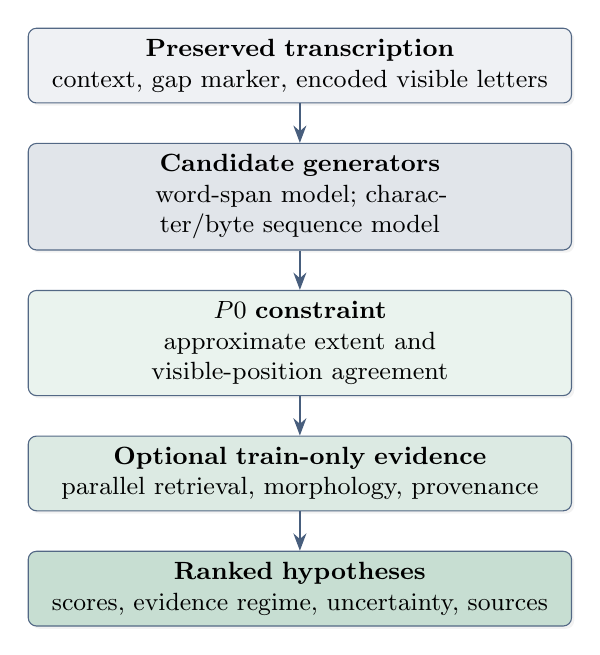
\begin{tikzpicture}[
  node distance=5mm,
  stage/.style={draw=DSSNavy!75,fill=DSSPaper,rounded corners=3pt,
    minimum width=6.9cm,text width=6.3cm,minimum height=8mm,
    align=center,inner sep=4pt,font=\small,
    drop shadow={opacity=0.10,shadow xshift=1pt,shadow yshift=-1pt}},
  flow/.style={-{Stealth[length=2.2mm]},line width=0.75pt,draw=DSSNavy!80}
]
\node[stage,fill=DSSNavy!7] (input) {\textbf{Preserved transcription}\\ context, gap marker, encoded visible letters};
\node[stage,fill=DSSNavy!13,below=of input] (gen) {\textbf{Candidate generators}\\ word-span model; character/byte sequence model};
\node[stage,fill=DSSEmerald!10,below=of gen] (constraint) {\textbf{$P0$ constraint}\\ approximate extent and visible-position agreement};
\node[stage,fill=DSSEmerald!17,below=of constraint] (rank) {\textbf{Optional train-only evidence}\\ parallel retrieval, morphology, provenance};
\node[stage,fill=DSSEmerald!27,below=of rank] (output) {\textbf{Ranked hypotheses}\\ scores, evidence regime, uncertainty, sources};
\draw[flow] (input) -- (gen);
\draw[flow] (gen) -- (constraint);
\draw[flow] (constraint) -- (rank);
\draw[flow] (rank) -- (output);
\end{tikzpicture}%
}
\caption{Proposed scholar-facing architecture. ``Visible letters'' are encoded from a transcription; the present system does not infer strokes directly from pixels.}
\label{fig:architecture}
\end{figure}

\section{Related Work}

\paragraph{Ancient-text restoration.}
Pythia introduced neural character restoration for Greek inscriptions and reported character error rate (CER) and Top-20 sequence recovery \cite{assael2019}. Recurrent models were also applied to fragmentary Babylonian texts \cite{fetaya2020}. Lazar et al.\ formulated Akkadian missing-sign completion as MLM inference and included expert evaluation \cite{lazar2021}. Ithaca combined character and word representations with attribution, dating, saliency, and a controlled historian study \cite{assael2022}. Aeneas subsequently integrated images, transcriptions, parallel retrieval, arbitrary-length restoration, and historian evaluation for Latin inscriptions \cite{assael2025}. The field-wide survey of Sommerschield et al.\ emphasizes that restoration must be located within a broader scholarly workflow \cite{sommerschield2023}.

\paragraph{Semitic and manuscript models.}
Embible ensembles character and word transformers for synthetically masked Biblical Hebrew and Aramaic \cite{fono2024}. MsBERT targets orthographic variation and lacunae in post-biblical Hebrew manuscripts \cite{shmidman2024}. TavBERT studies character-level pretraining for morphologically rich languages \cite{keren2022}; AlephBERT and DictaBERT provide strong Hebrew subword baselines \cite{seker2022,shmidman2023}. These models differ in period, register, tokenizer, and pretraining data, so a DSS comparison requires a shared target set and information condition.

\paragraph{Real lacunae and material evidence.}
The MAAT corpus preserves lacunae, restorations, and editorial structure from EpiDoc instead of reducing every example to random masking \cite{fitzgerald2024}. Levine et al.\ evaluate ranked, variable-length completions for Coptic manuscripts and explicitly frame predictions as scholar assistance \cite{levine2024}. For the DSS, Uzan et al.\ restore damaged letter images with a modified PixelCNN \cite{uzan2017}. That image-level task is complementary to our transcription-level span ranking; claims about ink or strokes require an explicit multimodal connection between them.

\section{Tasks and Information Conditions}

Let $x_{<g}$ and $x_{>g}$ be preserved context around a gap $g$. A system returns an ordered set $C_k(g)$ of at most $k$ complete strings. For synthetic damage with known preserved target $y_g$,
\begin{equation}
H_k(g)=\mathbb{I}[y_g\in C_k(g)].
\end{equation}
For a natural lacuna with a set $Y_g$ of distinct, bibliographically attributed proposals,
\begin{equation}
A_k(g)=\mathbb{I}[C_k(g)\cap Y_g\neq\varnothing].
\label{eq:agreement}
\end{equation}
$A_k$ is \emph{literature agreement}; neither inclusion nor exclusion establishes truth.

We distinguish three information conditions:

\begin{itemize}
  \item $U0$: context only; length, boundaries, and visible traces are unavailable.
  \item $O$-len: gold target length is supplied as an oracle diagnostic and cannot support a realistic headline claim.
  \item $P0$: approximate gap-derived length and transcription-encoded surviving letters are supplied. If $J$ indexes reliable visible positions, a candidate $c$ must satisfy $|c|\in[L-1,L+1]$ and $c_j=p_j$ for all $j\in J$.
\end{itemize}

The term ``material constraint'' is shorthand for information encoded by editors from the artifact. The current pipeline neither reads multispectral images nor estimates stroke probabilities.

\section{Data}

\paragraph{Corpus construction.}
The corpus is derived from the ETCBC DSS Text-Fabric dataset \cite{etcbcdss}. Biblical scrolls are excluded. Editorial reconstruction text is never emitted as a training label: physically preserved characters remain visible and gaps become anonymous \texttt{<GAP>} tokens. Deterministic scroll-level partitions contain 1,002 training, 238 development, and 407 held-out chunks. Corpus and lacuna files are recorded with SHA-256 hashes. Table~\ref{tab:corpus-overview} reports counts regenerated directly from the validated derivative.

\CorpusOverviewTable

\paragraph{What does a lacuna look like?}
The 27,814 records contain 165,239 damaged source-word positions (Table~\ref{tab:lacuna-shape}). Their median span is four positions, the 90th percentile is 13, and the maximum is 268. These are consecutive source-word positions after editorially supplied text has been removed. They describe the structure of the transcription and must not be read as 27,814 independent, metrically measured physical holes.

\LacunaShapeTable

The transcription nevertheless preserves useful material evidence. At least one word retains a visible trace in 23,632 lacuna records (85.0\%), but only 49,130 of the 165,239 damaged word positions (29.7\%) retain any trace. An estimated missing-character extent is available for 25,509 records (91.7\%); its median is five characters and its nearest-rank interquartile range is 2--12. Both left and right preserved context are available for 26,467 records (95.2\%), with a median of 14 total context words. The contrast between record-level evidence and position-level sparsity motivates constrained ranking without assuming that every hidden word has surviving ink.

\paragraph{Two evaluation views.}
No single benchmark answers both whether a system can recover a known string and whether it can surface a defensible proposal at a genuine lacuna. We therefore use the complementary views in Table~\ref{tab:evaluation-sets}: synthetic damage supplies an observable answer under controlled masking, while the QD set preserves natural ambiguity and supports only literature-agreement claims.

\EvaluationSetsTable

\paragraph{Synthetic alignment diagnostic.}
The shared 729-word diagnostic masks intact content words and tests whether candidate generation aligns with the same character interval. It is useful for tokenizer coverage, but it does not simulate unknown-length natural damage and is not the primary benchmark.

\paragraph{Unknown-length span pilot.}
We hide 300 preserved DSS spans, balanced across one, two, and three words, after fitting decoding parameters on 60 development spans. Character length, word count, and boundaries are hidden. Median character lengths are 3, 7, and 10 in the respective strata. The deterministic sample is nested with an earlier 30-span pilot and contains only six held-out scroll clusters. We report scroll-cluster bootstrap intervals, but their stability is limited by that small cluster count; this remains model-selection evidence rather than an independent test.

\paragraph{Qumran Digital targets.}
The QD snapshot dated 21 May 2026 contains 1,811 publication rows at 346 candidate locations. After predeclared exclusions, 74 non-biblical single-word targets remain across 37 scrolls, with 99 distinct physically compatible attributed readings. Twenty-two targets (29.7\%) have multiple attributed readings; estimated length has a median of five characters (range 2--9), and 72 targets retain a left or right edge anchor. Exclusions include multiword or incomplete readings, corrections, non-lacuna variants, insufficient context, unsupported markup, and proposals contradicting visible letters. The frozen manifest associated with the evaluated checkpoint assigns all 74 targets to held-out scrolls. A later registry instead assigns 40 of the 74 targets to train, 22 to validation, and 12 to test. The reported diagnostic is therefore held out relative to the checkpoint-associated split, but it must not be mixed with experiments trained under the later registry. Future training will freeze one authoritative registry before model fitting. QD selected disputed sites and is working scholarly data; the benchmark is neither random nor exhaustive.

\section{Models and Decoding}

\paragraph{Word-span baseline.}
The current leading implemented baseline enumerates one-token word hypotheses for unknown numbers of positions, combines forward and backward MLM evidence, and ranks complete surfaced strings. It is trained only on preserved non-biblical text. The tokenizer can represent 86.3\% of complete targets in the 300-span pilot; all others remain in the denominator.

\paragraph{Character and byte models.}
TavBERT supplies character-aligned masks, and a fine-tuned DictaBERT-char checkpoint provides a second character baseline. ByT5 supplies a byte-level sequence-to-sequence comparison \cite{raffel2020}. Character alignment avoids WordPiece drops, but alignment alone does not imply superior exact-span ranking.

\paragraph{Embible-style combinations.}
We implement both the paper-described overlap rule and a development-fitted rank fusion of word and character candidates. Under the locked tie-break, a simpler system is retained when exact Top-10 ties. This prevents selecting a more complex ensemble on secondary metrics alone.

\paragraph{Retrieval.}
The retrieval index contains preserved training scrolls only. Its weight is selected on development scrolls. Candidates are scored by the MLM plus a weighted exact-context signal. A final retrieval claim additionally requires answer-string removal, near-duplicate filtering, recall/MRR/nDCG reporting, and a paired downstream improvement with uncertainty.

\paragraph{Planned tokenization-free decoder.}
The promotion protocol requires a character-, byte-, or unrestricted span-sequence model that marginalizes or searches over output length and boundary hypotheses. Length-normalized scoring may be written as
\begin{equation}
s(c)=\frac{\sum_{i=1}^{|c|}\log p(c_i\mid c_{<i},x_{<g},x_{>g})}{|c|^{\alpha}},
\end{equation}
with $\alpha$ selected on development data. This component is a planned experiment, not the source of a reported success.

\section{Evaluation Protocol}

The primary automatic task is exact complete-span Top-10 under unknown length, word count, and word boundaries. Exact Top-1/5/20, MRR, CER, boundary F1, word-count mean absolute error, decoder failure, calibration, selective accuracy, and latency are secondary. Slot-level word hits are diagnostic only.

Scroll-disjoint is the minimum split; a composition-disjoint split is the hard evaluation. Formulaic and near-duplicate passages must be grouped before partitioning. Retrieval is restricted to training scrolls. Test data are never used for selection. Failed decoding, tokenizer misalignment, and unrepresentable targets count as misses.

Final experiments use seeds 41, 42, and 43, development-only early stopping, and a fixed tuning budget. We report seed variation and 95\% confidence intervals clustered by scroll (and composition in the hard split). System comparisons are paired at manuscript locations; multiplicity is corrected for the predeclared comparison family. Target-level predictions, exclusions, manifests, and code/data/model/result hashes are required for promotion. These reporting choices follow reproducibility guidance in NLP \cite{dodge2019,ulmer2024}.

\section{Pilot Results}

The results follow the task's sources of uncertainty rather than a leaderboard: we first test whether tokenization can align a known interval, then require exact recovery when length and boundaries are hidden, and finally measure agreement with attributed proposals at natural lacunae. Metrics are comparable only within each table.

\SyntheticAlignmentTable

\paragraph{Alignment is necessary but insufficient.}
Table~\ref{tab:alignment} uses a genuinely shared denominator. TavBERT base obtains the highest Hit@10, while DSS fine-tuning does not improve it. MsBERT's aligned-only rates are 9.78\% Hit@1 and 21.56\% Hit@10, but presenting those alone would condition on successful tokenization. With 279 of 729 failures counted as misses, its all-target rates are 6.04\% and 13.31\%. DictaBERT-char is omitted because the available 22.80\% result comes from a different 250-word pilot.

\SpanPilotTable
\SpanStrataTable

\paragraph{Unknown-length multiword restoration remains open.}
The preserved-only word-span model and rank fusion tie at 15.0\% exact Top-10 (Table~\ref{tab:spanpilot}); the simplicity rule retains the word model. The oracle word-length filter reaches 20.7\%, quantifying the benefit of unavailable structural information rather than a deployable gain. Table~\ref{tab:strata} exposes the decisive weakness: the baseline falls from 40.0\% on one-word spans to 5.0\% on two-word spans and 0.0\% on three-word spans. Coverage also degrades with length. Thus the pilot rejects, rather than validates, a claim of solved unknown-length restoration.

Three ByT5 checkpoints were also rerun on the identical target manifest. Each produces 0\% Top-10 on the two- and three-word strata. Because one checkpoint used different hyperparameters, these are checkpoint replications rather than a controlled three-seed estimate; their settings and target-level outputs remain in the frozen result artifacts.

\QDTable

\begin{figure}[t]
\centering
\resizebox{\linewidth}{!}{%
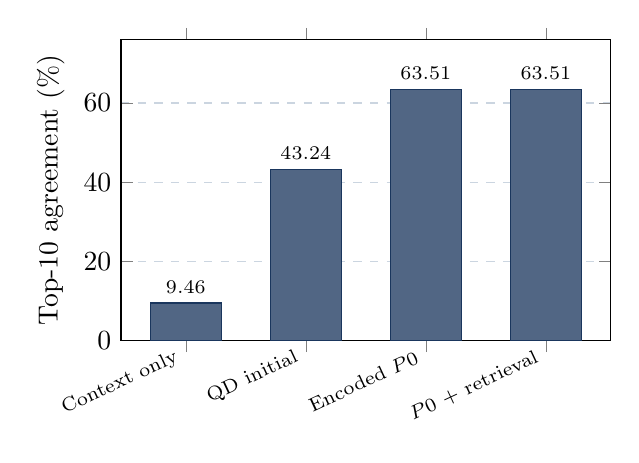
\begin{tikzpicture}
\begin{axis}[
  ybar,width=7.8cm,height=5.4cm,ymin=0,ymax=76,
  ylabel={Top-10 agreement (\%)},
  symbolic x coords={U0,Initial,P0,RAG},xtick=data,
  xticklabels={Context only,QD initial,Encoded $P0$,$P0$ + retrieval},
  x tick label style={rotate=25,anchor=east,font=\scriptsize},
  ytick={0,20,40,60},ymajorgrids=true,
  grid style={draw=DSSRule,dashed},bar width=9mm,enlarge x limits=0.18,
  nodes near coords,every node near coord/.append style={font=\scriptsize},
  nodes near coords align={vertical},clip=false
]
\addplot[draw=DSSNavy,fill=DSSNavy!76] coordinates
  {(U0,9.46) (Initial,43.24) (P0,63.51) (RAG,63.51)};
\end{axis}
\end{tikzpicture}%
}
\caption{QD Top-10 literature agreement. $U0$ and $P0$ use the same preserved-only MsBERT, isolating supplied evidence; the QD initial reading is contextual metadata, not a human control. Retrieval adds no test-set gain.}
\label{fig:qd-bars}
\end{figure}

\paragraph{Encoded constraints dominate within the QD diagnostic.}
On the same 74 targets, $P0$ changes Top-10 agreement from 9.5\% to 63.5\% (Table~\ref{tab:qd}). This paired input ablation shows that encoded constraints narrow candidates within this sample. The 95\% interval, clustered over 37 scrolls, is 52.4--74.4\%. The result is held out under the checkpoint-associated split, but is not comparable to models trained with the later registry. The 43.2\% QD initial-reading row describes overlap with an initial database reading and must not be interpreted as expert-alone performance. Exploratory character comparisons lack paired uncertainty and are therefore not promoted as evidence of a winner.

\paragraph{Retrieval is not yet a scoring contribution.}
Train-only retrieval leaves QD unchanged. Small positive Text-Fabric deltas use only 25 single-word spans or 100 multiword spans and assume known slot counts. They motivate a larger paired automatic evaluation but do not justify including retrieval in a champion system; the full ablation remains in the frozen result artifacts.

\section{Comparative Synthesis}

\SynthesisTable

Table~\ref{tab:synthesis} places the framework in its actual lineage. Lazar establishes ancient Semitic MLM completion; Embible motivates granularity ensembles; MsBERT motivates manuscript-domain pretraining; Aeneas demonstrates arbitrary-length multimodal restoration and controlled human evaluation. Our current contribution is an evaluation and evidence framework for DSS transcriptions. A final model contribution depends on passing the promotion gate.

\section{Reproducibility and Data Statement}

Core paper-facing numbers are regenerated from a frozen result snapshot containing target-manifest, model, input, and artifact hashes; a machine-readable table specification records evidence class and sources. The current snapshot reproduces the 300-span baselines and three ByT5 checkpoint evaluations on the same target hash, and reruns QD over 74 target-level records. The preserved corpus validator enforces non-biblical membership, removal of modern reconstruction text, anonymous gap representation, and disjoint splits. A leakage validator checks train/test scroll intersection, complete masking, and subtoken-length leakage. The protocol validator checks the frozen primary task and promotion criteria.

The camera-ready version will identify a pinned ETCBC DSS release and commit, QD snapshot date, licenses, model checkpoint revisions, parameter counts, training epochs, batch size, learning rate, optimizer, candidate-pool and beam sizes, tuning budget, software versions, hardware, elapsed time, and estimated compute. Anonymous review artifacts will contain no identity-bearing links. Public release remains subject to the licenses and attribution requirements of the source corpora and model checkpoints.

\section{Limitations and Responsible Use}

Synthetic damage preserves observable answers but differs from natural deterioration and editorial uncertainty. QD targets cover selected disputed sites, not a representative random sample, and its attributed proposals are incomplete. Text-Fabric editorial labels can encode modern reconstructions and therefore cannot serve as physical truth. Transcription-derived constraints inherit editor decisions about visible characters and gap extent. Period, dialect, genre, scribal practice, formulaic language, and orthography may all confound apparent model quality.

The current pilots are small, several are single-run, and most lack paired clustered intervals. The 300-span sample is nested with an earlier pilot. Retrieval may reproduce memorized parallels or editorial conventions. Character models solve alignment but have not solved exact multiword generation. Direct claims about ink require image inputs and image/transcription registration, which are absent here.

The system is intended for decision support. Every candidate should retain its model score, evidence condition, rejected constraints, provenance, and uncertainty. Suggestions must not be silently inserted into editions, used to overwrite attributed readings, or presented as recovered historical text. Scholars remain responsible for paleography, material joins, syntax, genre, parallels, and publication decisions.

\section{Conclusion}

The current evidence supports a narrower and more useful conclusion than the original roadmap claim. Character tokenization eliminates alignment drops, but does not automatically improve ranking. Transcription-derived material constraints substantially narrow a real-lacuna candidate space. Train-only retrieval has not yet improved QD agreement. Most importantly, exact unknown-length multiword restoration remains unsolved. The resulting protocol turns these observations into a reproducible research program: shared denominators, manuscript-disjoint data, exact complete-span scoring, paired uncertainty, and answer-removal tests.

\section*{Responsible NLP Research Checklist}

This draft follows the current ARR checklist structure \cite{arrchecklist}. Data provenance, language, licensing, exclusions, reconstruction redaction, and limitations are stated above. Final submission additionally requires completed compute/resource reporting, public artifact and model documentation, and statistical details. This work contains no human-participant study.

\begingroup
\small
\begin{thebibliography}{99}

\bibitem{assael2019}
Yannis Assael, Thea Sommerschield, and Jonathan Prag. 2019.
Restoring Ancient Text Using Deep Learning: A Case Study on Greek Epigraphy.
In \textit{Proceedings of EMNLP-IJCNLP}, pages 6368--6375.

\bibitem{assael2022}
Yannis Assael, Thea Sommerschield, Brendan Shillingford, Mahyar Bordbar,
John Pavlopoulos, Marita Chatzipanagiotou, Ion Androutsopoulos,
Jonathan Prag, and Nando de Freitas. 2022.
Restoring and Attributing Ancient Texts Using Deep Neural Networks.
\textit{Nature}, 603:280--283.

\bibitem{assael2025}
Yannis Assael, Thea Sommerschield, Alison Cooley, Brendan Shillingford,
John Pavlopoulos, Priyanka Suresh, Bailey Herms, Justin Grayston,
Benjamin Maynard, Nicholas Dietrich, Robbe Wulgaert, Jonathan Prag,
Alex Mullen, and Shakir Mohamed. 2025.
Contextualizing Ancient Texts with Generative Neural Networks.
\textit{Nature}, 645:141--147.

\bibitem{arrchecklist}
ACL Rolling Review. 2025.
Responsible NLP Research Checklist and Published Checklist Appendices.
\url{https://aclrollingreview.org/responsibleNLPresearch/}.

\bibitem{dodge2019}
Jesse Dodge, Suchin Gururangan, Dallas Card, Roy Schwartz, and Noah A. Smith. 2019.
Show Your Work: Improved Reporting of Experimental Results.
In \textit{Proceedings of EMNLP-IJCNLP}, pages 2185--2194.

\bibitem{etcbcdss}
Eep Talstra Centre for Bible and Computer. 2026.
The Dead Sea Scrolls in Text-Fabric.
Dataset and documentation, \url{https://github.com/ETCBC/dss}.

\bibitem{fetaya2020}
Ethan Fetaya, Yonatan Lifshitz, Elad Aaron, and Shai Gordin. 2020.
Restoration of Fragmentary Babylonian Texts Using Recurrent Neural Networks.
\textit{Proceedings of the National Academy of Sciences}, 117(37):22743--22751.

\bibitem{fitzgerald2024}
Will Fitzgerald and Justin Barney. 2024.
A New Machine-Actionable Corpus for Ancient Text Restoration.
In \textit{Proceedings of ML4AL}, pages 56--60.

\bibitem{fono2024}
Niv Fono, Harel Moshayof, Eldar Karol, Itai Assraf, and Mark Last. 2024.
Embible: Reconstruction of Ancient Hebrew and Aramaic Texts Using Transformers.
In \textit{Findings of EACL}, pages 846--852.

\bibitem{lazar2021}
Koren Lazar, Benny Saret, Asaf Yehudai, Wayne Horowitz, Nathan Wasserman,
and Gabriel Stanovsky. 2021.
Filling the Gaps in Ancient Akkadian Texts: A Masked Language Modelling Approach.
In \textit{Proceedings of EMNLP}, pages 4682--4691.

\bibitem{levine2024}
Lauren Levine, Cindy Li, Lydia Bremer-McCollum, Nicholas Wagner, and Amir Zeldes. 2024.
Lacuna Language Learning: Leveraging RNNs for Ranked Text Completion in Digitized Coptic Manuscripts.
In \textit{Proceedings of ML4AL}, pages 61--70.

\bibitem{raffel2020}
Colin Raffel, Noam Shazeer, Adam Roberts, Katherine Lee, Sharan Narang,
Michael Matena, Yanqi Zhou, Wei Li, and Peter J. Liu. 2020.
Exploring the Limits of Transfer Learning with a Unified Text-to-Text Transformer.
\textit{Journal of Machine Learning Research}, 21(140):1--67.

\bibitem{keren2022}
Omri Keren, Tal Avinari, Reut Tsarfaty, and Omer Levy. 2022.
Breaking Character: Are Subwords Good Enough for MRLs After All?
\textit{arXiv preprint arXiv:2204.04748}.

\bibitem{seker2022}
Amit Seker, Elron Bandel, Dan Bareket, Idan Brusilovsky, Refael Greenfeld,
and Reut Tsarfaty. 2022.
AlephBERT: Language Model Pre-training and Evaluation from Sub-Word to Sentence Level.
In \textit{Proceedings of ACL}, pages 46--56.

\bibitem{shmidman2023}
Avi Shmidman, Shaltiel Shmidman, Moshe Koppel, and Yoav Goldberg. 2023.
DictaBERT: A State-of-the-Art BERT Suite for Modern Hebrew.
\textit{arXiv preprint arXiv:2308.16687}.

\bibitem{shmidman2024}
Avi Shmidman, Ometz Shmidman, Hillel Gershuni, and Moshe Koppel. 2024.
MsBERT: A New Model for the Reconstruction of Lacunae in Hebrew Manuscripts.
In \textit{Proceedings of ML4AL}, pages 13--18.

\bibitem{sommerschield2023}
Thea Sommerschield, Yannis Assael, John Pavlopoulos, Vanessa Stefanak,
Andrew Senior, Chris Dyer, John Bodel, Jonathan Prag, Ion Androutsopoulos,
and Nando de Freitas. 2023.
Machine Learning for Ancient Languages: A Survey.
\textit{Computational Linguistics}, 49(3):703--747.

\bibitem{ulmer2024}
Nicholas Lourie, Kyunghyun Cho, and He He. 2024.
Show Your Work with Confidence: Confidence Bands for Tuning Curves.
In \textit{Proceedings of NAACL}, pages 3455--3472.

\bibitem{uzan2017}
Lior Uzan, Nachum Dershowitz, and Lior Wolf. 2017.
Qumran Letter Restoration by Rotation and Reflection Modified PixelCNN.
In \textit{Proceedings of ICDAR}, pages 23--29.

\end{thebibliography}
\endgroup

\end{document}
